\documentclass{article}

% packages
\usepackage{amsmath, amsthm, thmtools, amsfonts, amssymb, luacode, catchfile, tikzducks, hyperref, ifthen}
\ifcsname c@kobocompile\endcsname
	\usepackage[a5paper, total={1072pt, 1448pt}, margin=10pt, includeheadfoot]{geometry} % set page margins
\else
	\usepackage[a4paper, margin=50pt, includeheadfoot]{geometry}
\fi
\usepackage[shortlabels]{enumitem}
\usepackage[skip=3pt, indent=0pt]{parskip}

% language
\usepackage[bidi=basic, layout=tabular, provide=*]{babel}
\ifcsname c@english\endcsname
	\babelprovide[main, import]{english}
\else
	\babelprovide[main, import]{hebrew}
	\babelprovide{rl}
\fi
%\babelfont{rm}{Libertinus Serif}
\babelfont{rm}[Renderer=Harfbuzz]{Libertinus Serif}
\babelfont{sf}{Libertinus Sans}
\babelfont{tt}{Libertinus Mono}

% style
\AddToHook{cmd/section/before}{\clearpage}	% Add line break before section
\linespread{1.3}
\setcounter{secnumdepth}{0}		% Remove default number tags from sections, this won't do well with theorems
\AtBeginDocument{\setlength{\belowdisplayskip}{3pt}}
\AtBeginDocument{\setlength{\abovedisplayskip}{3pt}}
\graphicspath{ {../images/} }

% operators
\DeclareMathOperator\cis{cis}
\DeclareMathOperator\Sp{Sp}
\DeclareMathOperator\tr{tr}
\DeclareMathOperator\im{Im}
\DeclareMathOperator\re{Re}
\DeclareMathOperator\diag{diag}
\DeclareMathOperator*\lowlim{\underline{lim}}
\DeclareMathOperator*\uplim{\overline{lim}}
\DeclareMathOperator\rng{rng}
\DeclareMathOperator\Sym{Sym}
\DeclareMathOperator\Arg{Arg}
\DeclareMathOperator\Log{Log}
\DeclareMathOperator\dom{dom}
\DeclareMathOperator\supp{Supp}
\DeclareMathOperator\var{Var}
\DeclareMathOperator\cov{Cov}

% commands
%\renewcommand\qedsymbol{\textbf{מש''ל}}
%\renewcommand\qedsymbol{\fbox{\emoji{lizard}}}
\newcommand{\Aa}[0]{\mathcal{A}}
\newcommand{\Bb}[0]{\mathcal{B}}
\newcommand{\CC}[0]{\mathbb{C}}
\newcommand{\Cc}[0]{\mathcal{C}}
\newcommand{\EE}[0]{\mathbb{E}}
\newcommand{\FF}[0]{\mathbb{F}}
\newcommand{\Ff}[0]{\mathcal{F}}
\newcommand{\Ii}[0]{\mathcal{I}}
\newcommand{\Gg}[0]{\mathcal{G}}
\newcommand{\Ll}[0]{\mathcal{L}}
\newcommand{\Mm}[0]{\mathcal{M}}
\newcommand{\NN}[0]{\mathbb{N}}
\newcommand{\Nn}[0]{\mathcal{N}}
\newcommand{\PP}[0]{\mathbb{P}}
\newcommand{\Pp}[0]{\mathcal{P}}
\newcommand{\QQ}[0]{\mathbb{Q}}
\newcommand{\RR}[0]{\mathbb{R}}
\newcommand{\Rr}[0]{\mathcal{R}}
\newcommand{\Ss}[0]{\mathcal{S}}
\newcommand{\TT}[0]{\mathbb{T}}
\newcommand{\Uu}[0]{\mathcal{U}}
\newcommand{\Vv}[0]{\mathcal{V}}
\newcommand{\Ww}[0]{\mathcal{W}}
\newcommand{\ZZ}[0]{\mathbb{Z}}
\newcommand{\acts}[0]{\circlearrowright}
\newcommand{\explain}[2] {
	\begin{flalign*}
		 && \text{#2} && \text{#1}
	\end{flalign*}
}
\newcommand{\maketitleprint}[0]{ \begin{center}
	%\begin{tikzpicture}[scale=3]
	%	\duck[graduate=gray!20!black, tassel=red!70!black]
	%\end{tikzpicture}	
	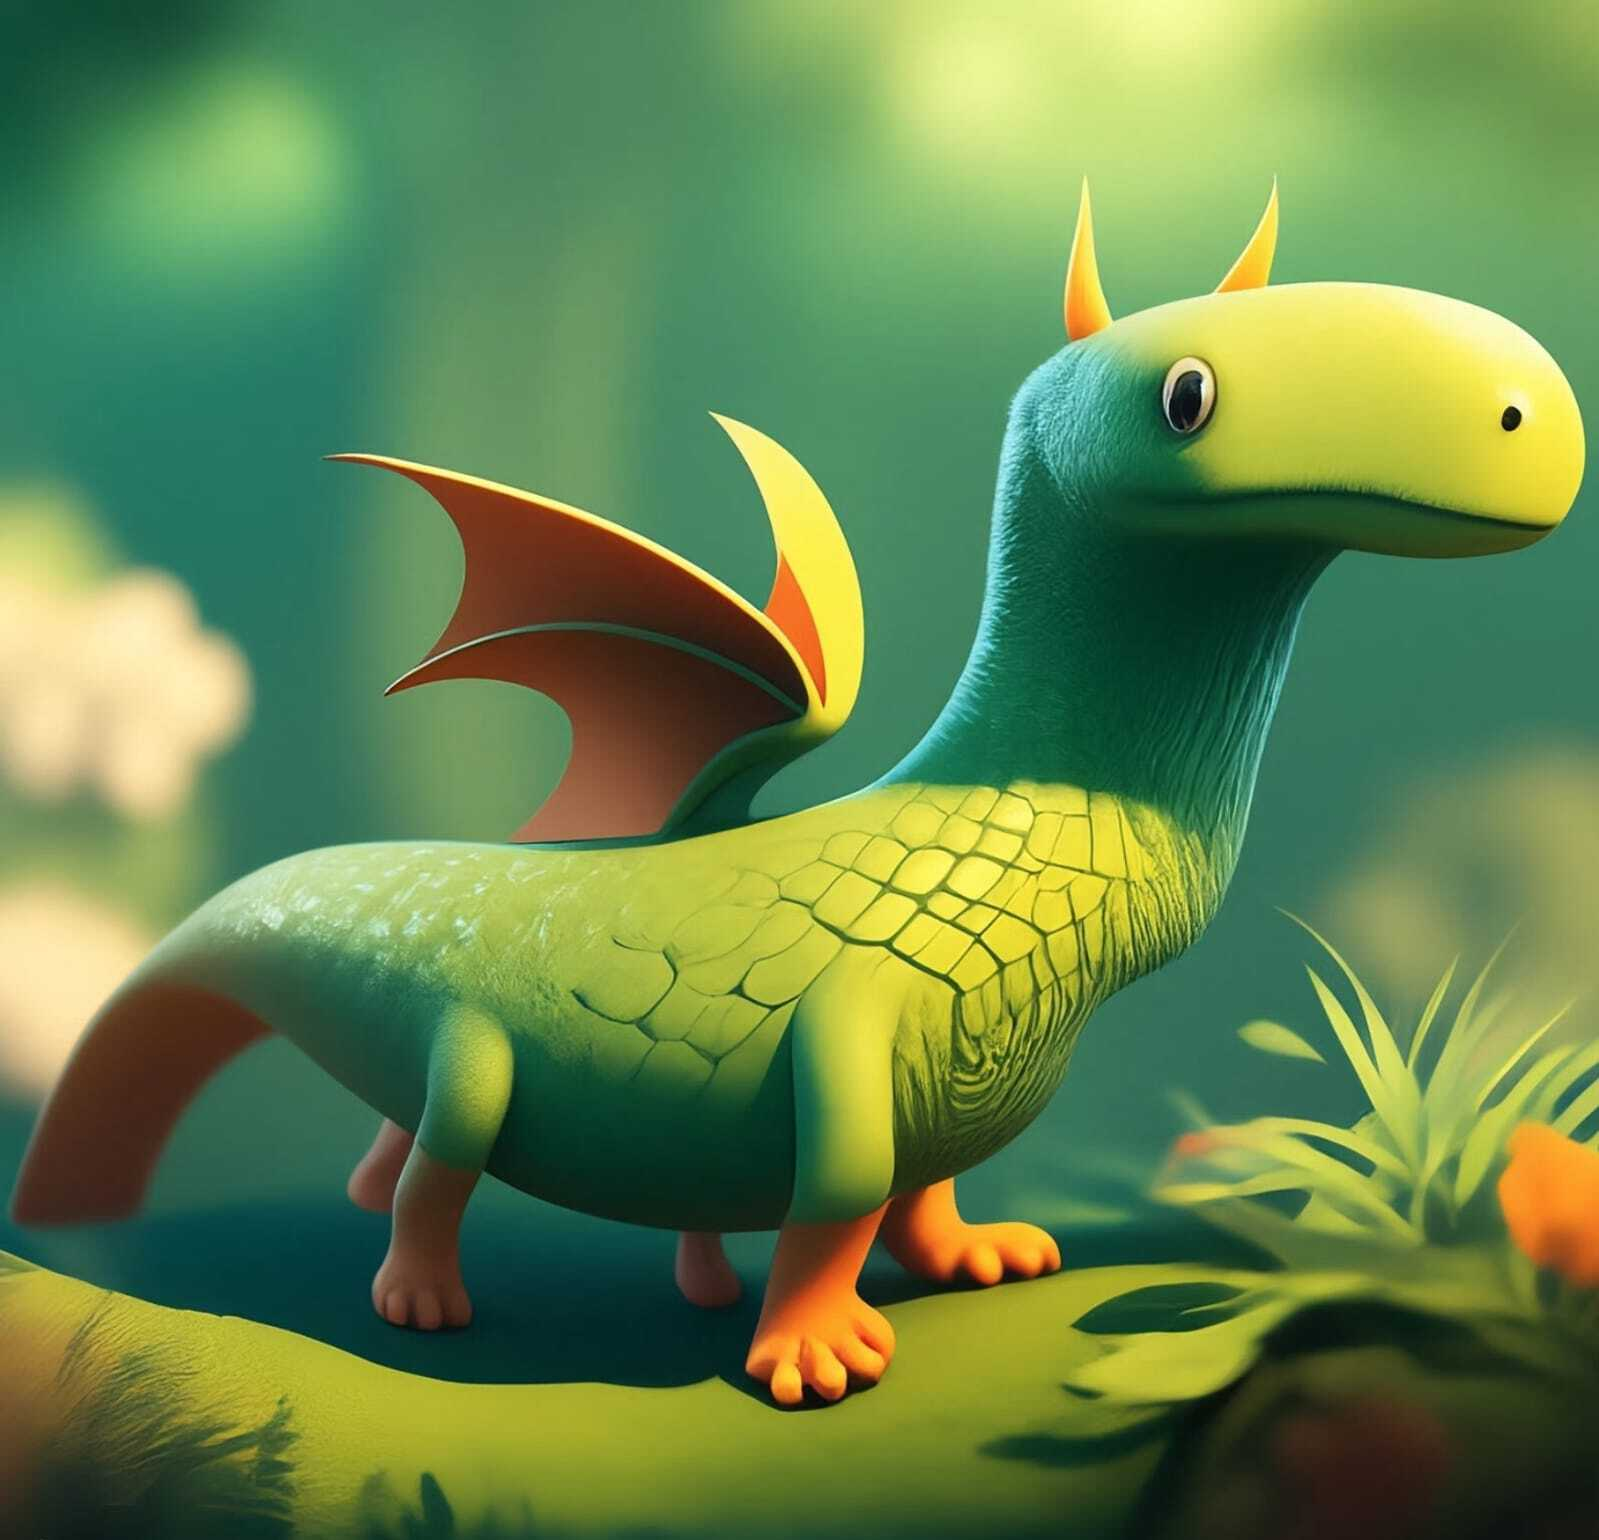
\includegraphics[width=6cm]{cover}
\end{center}
}

% theorem commands
\newtheoremstyle{c_remark}
	{}	% Space above
	{}	% Space below
	{}% Body font
	{}	% Indent amount
	{\bfseries}	% Theorem head font
	{}	% Punctuation after theorem head
	{.5em}	% Space after theorem head
	{\thmname{#1}\thmnumber{ #2}\thmnote{ \normalfont{\text{(#3)}}}}	% head content
\newtheoremstyle{c_definition}
	{3pt}	% Space above
	{3pt}	% Space below
	{}% Body font
	{}	% Indent amount
	{\bfseries}	% Theorem head font
	{}	% Punctuation after theorem head
	{.5em}	% Space after theorem head
	{\thmname{#1}\thmnumber{ #2}\thmnote{ \normalfont{\text{(#3)}}}}	% head content
\newtheoremstyle{c_plain}
	{3pt}	% Space above
	{3pt}	% Space below
	{\itshape}% Body font
	{}	% Indent amount
	{\bfseries}	% Theorem head font
	{}	% Punctuation after theorem head
	{.5em}	% Space after theorem head
	{\thmname{#1}\thmnumber{ #2}\thmnote{ \text{(#3)}}}	% head content

\ifcsname c@english\endcsname
	\theoremstyle{plain}
	\newtheorem{theorem}{Theorem}[section]
	\newtheorem{lemma}[theorem]{Lemma}
	\newtheorem{proposition}[theorem]{Proposition}
	\newtheorem*{proposition*}{Proposition}
	%\newtheorem{corollary}[theorem]{אין חלופה עברית}

	\theoremstyle{definition}
	\newtheorem{definition}[theorem]{Definition}
	\newtheorem*{definition*}{Definition}
	\newtheorem{example}{Example}[section]
	\newtheorem{exercise}{Exercise}[section]

	\theoremstyle{remark}
	\newtheorem*{remark}{Remark}
	\newtheorem*{solution}{Solution}
	\newtheorem{conclusion}[theorem]{Conclusion}
	\newtheorem{notation}[theorem]{Notation}
\else
	\theoremstyle{c_plain}
	\newtheorem{theorem}{משפט}[section]
	\newtheorem{lemma}[theorem]{למה}
	\newtheorem{proposition}[theorem]{טענה}
	\newtheorem*{proposition*}{טענה}
	%\newtheorem{corollary}[theorem]{אין חלופה עברית}

	\theoremstyle{c_definition}
	\newtheorem{definition}[theorem]{הגדרה}
	\newtheorem*{definition*}{הגדרה}
	\newtheorem{example}{דוגמה}[section]
	\newtheorem{exercise}{תרגיל}[section]

	\theoremstyle{c_remark}
	\newtheorem*{remark}{הערה}
	\newtheorem*{solution}{פתרון}
	\newtheorem{conclusion}[theorem]{מסקנה}
	\newtheorem{notation}[theorem]{סימון}
\fi

% Questions related commands
\newcounter{question}
\setcounter{question}{1}
\newcounter{sub_question}
\setcounter{sub_question}{1}

\ifcsname c@english\endcsname
	\newcommand{\question}[1][0]{
		\ifthenelse{#1 = 0}{}{\setcounter{question}{#1}}
		\section{Question \arabic{question}}
		\addtocounter{question}{1}
		\setcounter{sub_question}{1}
	}

	\newcommand{\subquestion}[1][0]{
		\ifthenelse{#1 = 0}{}{\setcounter{sub_question}{#1}}
		\subsection{Part \alph{sub_question}}
		\addtocounter{sub_question}{1}
	}
\else
	\newcommand{\question}[1][0]{
		\ifthenelse{#1 = 0}{}{\setcounter{question}{#1}}
		\section{שאלה \arabic{question}}
		\addtocounter{question}{1}
		\setcounter{sub_question}{1}
	}

	\newcommand{\subquestion}[1][0]{
		\ifthenelse{#1 = 0}{}{\setcounter{sub_question}{#1}}
		\subsection{סעיף \localecounter{letters.gershayim}{sub_question}}
		\addtocounter{sub_question}{1}
	}
\fi

% import lua and start of document
\directlua{common = require ('../common')}

\GetEnv{AUTHOR}

% headers
\author{\AUTHOR}
\date\today

\title{פתרון מטלה 04 --- חשבון אינפינטסמלי 3 (80415)}

\begin{document}
\maketitle
\maketitleprint{}

\Question{}
נוכיח מהגדרה כי הפונקציות הבאות הן דיפרנציאביליות ונמצא את הדיפרנציאל שלהן.

\Subquestion{}
תהי $T : \RR^k \to \RR^m$ העתקה לינארית ו־$b \in \RR^m$, ונבדוק את הפונקציה $f : \RR^k \to \RR^m$ המוגדרת על־ידי
\[
	f(x) = Tx + b
\]

נבחין כי
\[
	\lim_{v \to 0} \frac{f(x + v) - f(x) - Sv}{\lVert v \rVert}
	= \lim_{v \to 0} \frac{T(x + v) + b - Tx - b - Sv}{\lVert v \rVert}
	= \lim_{v \to 0} \frac{Tv - Sv}{\lVert v \rVert}
\]
ונבחין כי עבור $S = T$ גבול זה אכן מתקיים, ולכן $f$ דיפרנציאבילית בכל נקודה ונגזרתה $T$.

\Subquestion{}
תהי $g : \RR^k \to \RR$ המוגדרת על־ידי
\[
	g(x) = \lVert x \rVert^2 = \langle x, x \rangle
\]

נבדוק את הגבול כאשר נגדיר את הנורמה להיות מכפלה פנימית:
\begin{align*}
	\lim_{v \to 0} \frac{g(x + v) - g(x) - Tv}{\lVert v \rVert}
	& = \lim_{v \to 0} \frac{\langle x + v, x + v \rangle - \lVert x \rVert^2 - Tv}{\lVert v \rVert} \\
	& = \lim_{v \to 0} \frac{\lVert x \rVert^2 + \lVert v \rVert^2 + 2\langle x, v \rangle - \lVert x \rVert^2 - Tv}{\lVert v \rVert} \\
	& = \lim_{v \to 0} \frac{\lVert v \rVert^2 + 2\langle x, v \rangle - Tv}{\lVert v \rVert} \\
	& = \lim_{v \to 0} \lVert v \rVert + \frac{2\langle x, v \rangle - Tv}{\lVert v \rVert} \\
\end{align*}
ונקבל כי הגבול מתקיים אילו $T = 2x$ ובהתאם $Tv = \langle x, v \rangle$.

\Question{}
תהי פונקציה $f : \RR^n \to \RR^m$ ונסמן ב־$f_1, \dots, f_m$ את רכיביה.
תהי $p \in \RR^n$.
נוכיח ש־$f$ גזירה אם ורק אם כל הרכיבים שלה גזירים ב־$p$.
\begin{proof}
	\textbf{כיוון ראשון:}
	נניח כי $f$ גזירה ב־$p$ ותהי $T$ נגזרת שלה, לכן מתקיים
	\[
		\lim_{v \to 0} \frac{f(p + v) - f(p) - Tv}{\lVert v \rVert} = 0
	\]
	אנו יודעים כי העתקות לינאריות משרות נורמות מהמטלה הקודמת ולכן נוכל לקבוע כי עבור העתקה לינארית $S : \RR^m \to \RR$ כי
	\[
		\lim_{v \to 0} S(\frac{f(p + v) - f(p) - Tv}{\lVert v \rVert}) = 0
		\implies
		\lim_{v \to 0} \frac{S f(p + v) - S f(p) - STv}{\lVert v \rVert} = 0
	\]
	עתה נגדיר $S = \pi_i$ עבור $1 \le i \le m$ ונקבל
	\[
		\lim_{v \to 0} \frac{f_i(p + v) - f_i(p) - {(Tv)}_i}{\lVert v \rVert} = 0
	\]
	בפרט עבור $t \in \RR$ מתקיים
	\[
		\lim_{t \to 0} \frac{f_i(p + te_i) - f_i(p) - |t| {(Te_i)}_i}{|t|} = 0
	\]
	והגדרת הנגזרת מתקיימת ונקבל $f_i'(t) = {(Te_i)}_i$.

	\textbf{כיוון שני:}
	נניח כי $f_i$ גזירה לכל $1 \le i \le m$ ונסמן $T_i : \RR^n \to \RR$ נגזרת זו. \\*
	נגדיר $T : \RR^n \to \RR^m$ התעתקה לינארית המוגדרת על־ידי $T v = {(T_1 v, T_2 v, \dots, T_m v)}^t$.
	עתה נבחן את הגבול
	\begin{align*}
		\lim_{v \to 0} \frac{f(p + v) - f(p) - Tv}{\lVert v \rVert}
		& = \lim_{v \to 0} \frac{f(p + v) - f(p) - Tv}{\lVert v \rVert} \\
		& = \lim_{v \to 0} \frac{{(f_1(p + v) - f_1(p) - T_1 v, \dots, f_m(p + v) - f_m(p) - T_m v)}^t}{\lVert v \rVert} \\
		& = \lim_{v \to 0} {\left( \frac{f_1(p + v) - f_1(p) - T_1 v}{\lVert v\rVert}, \dots, \frac{f_m(p + v) - f_m(p) - T_m v}{\lVert v\rVert}\right)}^t
		& = {(0, \dots, 0)}^t
	\end{align*}
	התכנסות בנפרד בכלל האגפים על־פי הגדרות הנגזרות $T_i$ וקיבלנו כי $T$ דיפרנציאל של $f$ ב־$p$.
\end{proof}

\Question{}
\Subquestion{}
נוכיח שאם $f : \RR^n \to \RR^m$ גזירה בנקודה $p \in \RR^n$ אז היא רציפה ב־$p$.
\begin{proof}
	נניח כי $f$ גזירה ב־$p$ ונגזרתה $T$, לכן
	\[
		\lim_{v \to 0} \frac{f(p + v) - f(p) - Tv}{\lVert v \rVert} = 0
	\]
	ואנו יודעים כי $\lVert v \rVert \xrightarrow{v \to 0} 0$ ולכן גם
	\[
		\lim_{v \to 0} \lVert v \rVert \cdot \frac{f(p + v) - f(p) - Tv}{\lVert v \rVert}
		= \lim_{v \to 0} \cdot f(p + v) - f(p) - Tv
		= 0
	\]
	אבל אנחנו יודעים השיעור כי $Tv \xrightarrow{v \to 0} 0$ ולכן בהכרח
	\[
		\lim_{v \to 0} \cdot f(p + v) - f(p) - Tv
		\lim_{v \to 0} \cdot f(p + v) - f(p)
		= 0
	\]
	ונקבל בהתאם גם כי
	\[
		\lim_{v \to p} \cdot f(v) = f(p)
	\]
	דהינו הפונקציה רציפה ב־$p$.
\end{proof}

\Subquestion{}
נוכיח כי אם $f, g : \RR^n \to \RR^m$ גזירות בנקודה $p$ אז גם $f + g$ גזירה בנקודה זו ומתקיים $D(f + g)\mid_p = Df\mid_p + Dg\mid_p$.
\begin{proof}
	נגדיר $T, S$ נגזרות $f, g$ בהתאמה בנקודה $p$, לכן מתקיים
	\[
		\lim_{v \to 0} \frac{f(p + v) - f(p) - Tv}{\lVert v \rVert},
		\lim_{v \to 0} \frac{g(p + v) - g(p) - Sv}{\lVert v \rVert}
	\]
	ולכן נוכל לחבר את הגבולות ונקבל
	\begin{align*}
		& \lim_{v \to 0} \frac{f(p + v) - f(p) - Tv}{\lVert v \rVert} + \frac{g(p + v) - g(p) - Sv}{\lVert v \rVert}
		& & = \lim_{v \to 0} \frac{f(p + v) - f(p) - Tv + g(p + v) - g(p) - Sv}{\lVert v \rVert} \\
		& = \lim_{v \to 0} \frac{(f + g)(p + v) - (f(p) + g(p)) - (T + S)v}{\lVert v \rVert}
		& & = D(f + g)\mid_p = Df\mid_p + Dg\mid_p
	\end{align*}
\end{proof}

\Question{}
\Subquestion{}
תהי $f : \RR^3 \to \RR^2$ המוגדרת על־ידי
\[
	f(x, y, z) = (x^2 y^3 z^4, x^8 - \cos(xy))
\]

נמצא את נגזרתה של $f$.
\[
	Df = \begin{pmatrix}
		2 x y^3 z^4 & 8x^7 + y \sin(xy) \\
		3 x^2 y^2 z^4 & x \sin(xy) \\
		4 x^2 y^3 z^3 & 0
	\end{pmatrix}
\]
נשים לב כי $f$ מוגדרת על־ידי פונקציות רציפות וגזירות ולכן גם היא רציפה וגזירה בכל תחומה.

\Subquestion{}
נגדיר $f : \RR^2 \to \RR$ על־ידי
\[
	f(x, y) = \begin{cases}
		x^\frac{n}{5} \sin(\frac{y}{x}) & x \ne 0 \\
		0 & x = 0
	\end{cases}
\]
נמצא את הערכים של $n \in \NN$ עבורם הפונקציה גזירה ב־$(0, 0)$.

נתחיל במציאת $Df$ ב־$\RR^2 \setminus\{(0, 0)\}$:
\begin{align*}
	Df & = \left( \frac{n}{5}x^{\frac{n}{5} - 1} \sin(\frac{y}{x}) + x^\frac{n}{5} \cos(\frac{y}{x}) \cdot \frac{-y}{x^2}, x^\frac{n}{5} \cos(\frac{y}{x}) \cdot \frac{1}{x} \right) \\
	   & = \left( \frac{n}{5}x^{\frac{n}{5} - 1} \sin(\frac{y}{x}) - x^{\frac{n}{5} - 1} y \cos(\frac{y}{x}), x^{\frac{n}{5} - 1} \cos(\frac{y}{x}) \right)
\end{align*}
ועלינו למצוא ערכי $n$ כך שהפונקציה רציפה באפס.
נשים לב כי כלל איברי שני הביטויים הם מכפלה של $x^{\frac{n}{5} - 1}$ והם ביטויים חסומים או אפסות ($y$), ולכן מספיק שיתקיים $x^{\frac{n - 5}{5}} \xrightarrow{x \to 0} 0$. \\*
גבול זה כמובן מתקיים כל תנאי ש־$n \ne 5$, ולכן התנאי ההכרחי לגזירות $f$ ב־$(0, 0)$ הוא $n \ne 5$.

\Question{}
\Subquestion{}
זבוב נמצא בנקודה $p = (0, 0, 5)$ בחדר שהטמפרטורה בו נתונה על־ידי הפונקציה
\[
	T(x, y, z) = e^x + 2y + z^2 - 7z
\]
נמצא את הווקטור אליו יעוף הזבוב כדי להתחמם.

נחשב תחילה את הגרדיאנט של $T$ בנקודה.
\[
	DT = (e^x, 2, 2z - 7)
\]
ובהתאם נציב ונקבל כי $\nabla p = (1, 2, 3)$. \\*
לכן עלינו למצוא $v \in \RR^3$ כך ש־$\langle \nabla p, v \rangle > 0$, ונקבל $\{ \frac{1}{\sqrt{5t^2 + 2ts + 10s^2}}(-2t - 3s, t, s) \mid s, t > 0 \}$. \\*
כדי להתחמם במהירות הגבוהה ביותר הזבוב יבחר את הכיוון $(0, 0, 1)$.

\Subquestion{}
תהי נמלה המוכלת בשולחן המוגדר על־ידי $z = 5$, נחשב את הכיוון אליו היא צריכה ללכת כדי להתחמם.

נשים לב כי נוכל להשתמש בקבוצת הפתרונות מהסעיף הקודם ולהציב $s = 0$ ולקבל כי עליה ללכת בכיוון $(0, 1, 0)$ (כך היא אכן לא תצטרך לעוף, ואין סתירה לנתון כי היא איננה מעופפת). \\*
נוכל כמובן גם להגדיר פונצקיה חדשה על־ידי $\tilde{T}(x, y) = T(x, y, 5) = e^x + 2y + 3$ ונקבל עבורה $\nabla \tilde{T} p = (4, 5)$ ומכאן נסיק ישירות כי עליה ללכת בכיוון $(1, 0)$ או $(0, 1)$ או כל שילוב חיובי שלהם.

\Question{}
נגדיר
\[
	f(x, y) = \begin{cases}
		\frac{x^3}{x^2 + y^2} & (x, y) \ne (0, 0) \\
		0 & (x, y) = (0, 0)
	\end{cases}
\]

\Subquestion{}
עבור כל $v = (a, b) \in \RR^2$ נראה שהנגזרת המכוונת $\partial_v f \mid_{(0, 0)}$ קיימת ונחשב אותה.

\[
	\partial_v f \mid_{(0, 0)}
	= \lim_{t \to 0} \frac{f(t v) - t(0)}{\lVert t v \rVert}
	= \lim_{t \to 0} \frac{\frac{t^3 a^3}{t^2 (a^2 + b^2)} - 0}{t}
	= \lim_{t \to 0} \frac{t^3 a^3 - 0}{t^3 (a^2 + b^2)}
	= \frac{a^3}{a^2 + b^2}
\]
ומצאנו כי הנגזרת המכוונת לכל כיוון ב־$(0, 0)$ מוגדרת.

\Subquestion{}
נוכיח ש־$f$ לא גזירה ב־$(0, 0)$.
\begin{proof}
	נניח בשלילה ש־$f$ גזירה בנקודה $(0, 0)$ ונניח כי $T$ הנגזרת בנקודה. \\*
	בסעיף הקודם מצאנו נגזרת מכוונת ולכן נשתמש בה כדי למצוא את ערכי המטריצה מסד$2 \times 1$ המייצגת את $T$. \\*
	תחילה נבדוק את $(0, 1)$, הצבתו בנגזרת המכוונת מציבה $\partial_{(0, 1)} f |_{(0, 0)} = 0$ ולכן $T(0, 1) = 0$. \\*
	עוד נקבל כי $\partial_{(1, 0)} f |_{(0, 0)} = 1$ ובהתאם $T(1, 0) = 1$ ונוכל להסיק כי $T = (1, 0)$. \\*
	נציב שוב עבור $(1, 1)$ ונקבל בהתאם $T(1, 1) = \frac{1}{2}$ בסתירה לזה שמצאנו כי $T(1, 1) = T(1, 0) + T(0, 1) = 1$. \\*
	נוכל אם כן להסיק שהעתקה זו לא קיימת ובהתאם $f$ לא דיפרנציאבילית בנקודה.
\end{proof}

\end{document}
